\documentclass{article}

\usepackage[a4paper, bottom=0.5in, top=0.5in, left=0.5in, right=0.5in]{geometry}
\usepackage{wrapfig}
\usepackage{natbib}
\usepackage{url}
\usepackage{xcolor}
\usepackage{caption}
\usepackage{hyperref}
\hypersetup{
    colorlinks=true,    
    urlcolor=cyan,
}
\usepackage{bytefield}

\usepackage{amsfonts}
\usepackage{float}
\usepackage{enumitem}

\usepackage{tikz-timing}[2014/10/29]
\usetikztiminglibrary[rising arrows]{clockarrows}

\usepackage{minted}

\usepackage{xparse} % NewDocumentCommand, IfValueTF, IFBooleanTF
\usepackage{tikz-timing}[2014/10/29]
\NewDocumentCommand{\busref}{som}{\texttt{%
		#3%
		\IfValueTF{#2}{[#2]}{}%
		\IfBooleanTF{#1}{\#}{}%
}}


\newcommand{\bitFormat}[1]{\emph{\textbf{\textcolor{cyan}{#1}}}}

\newcommand{\regFormat}[1]{\textbf{\textcolor{magenta}{#1}}}

\newcommand{\pinFormat}[1]{\emph{\textcolor{red}{#1}}}


\usepackage{graphicx}
\graphicspath{ {./Resources/pics/} }



\title{ATmega328P SPI}
\author{Narendiran S}
\date{\today}

\begin{document}
\maketitle

\section{Features}
\begin{itemize}
    \item Full-duplex, three-wire synchronous data transfer
    \item LSB first or MSB first
    \item Seven Programmable bit rates
    \item high-speed synchronous data transfe
\end{itemize}

\section{Block Diagram}
\begin{figure}[H]
    \centering
    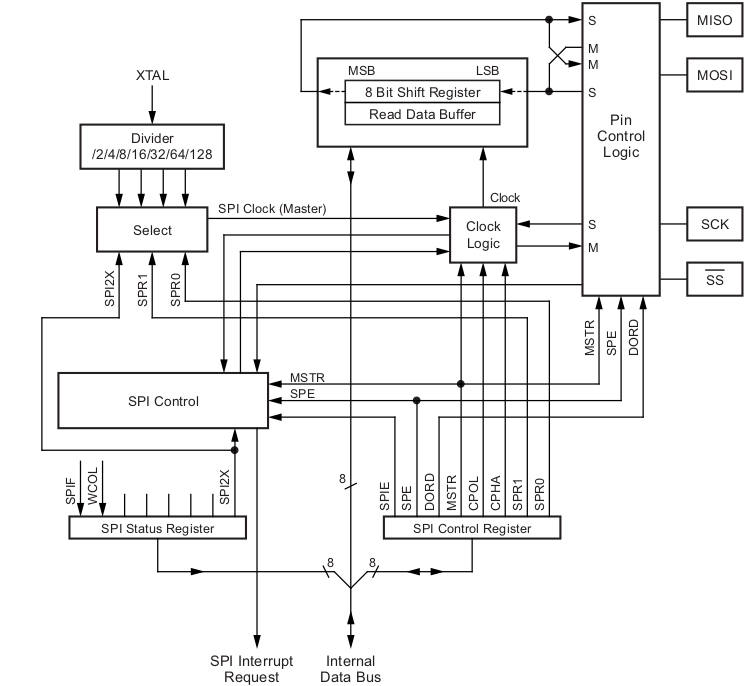
\includegraphics[height=0.6\textheight]{SPIBlockDiagram.png}
\end{figure}

\section{SPI Master-Slave Interconnection}
\begin{figure}[H]
    \centering
    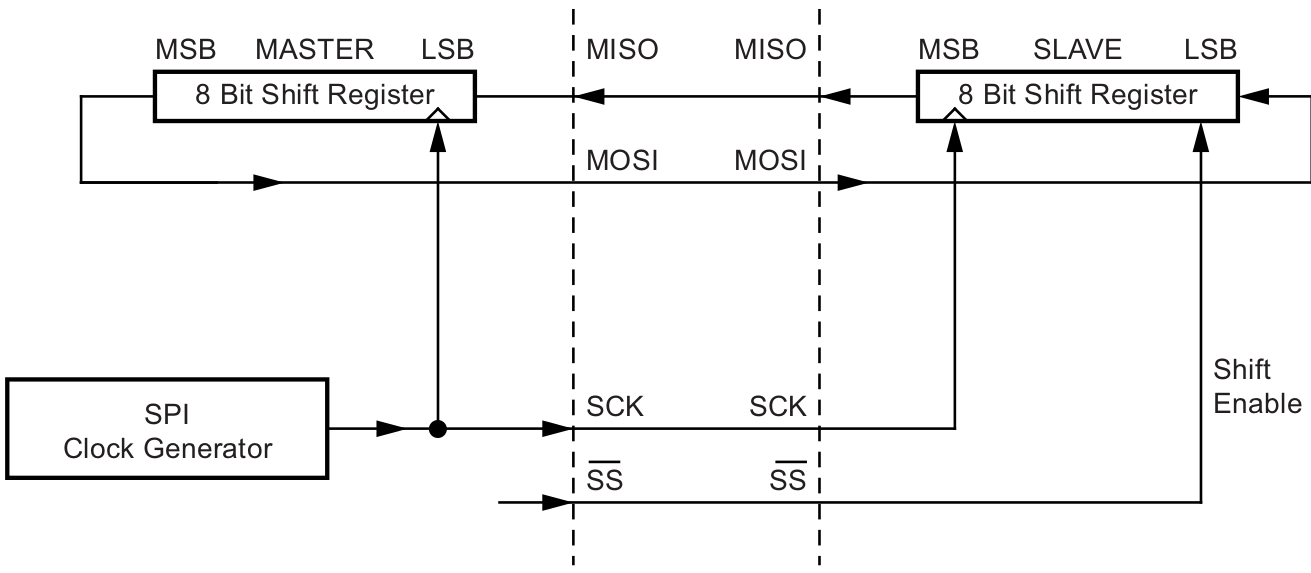
\includegraphics[width=0.6\textwidth]{SPIInterconnection.png}
\end{figure}
\subsection{SPI Pins}
\quad The SPI is connected to external devices trhough four pins namely,
\begin{itemize}
	\item \textbf{MISO} - Master IN / Slave OUT data - transmit data in slave mode and receive data in master mode.
	\item \textbf{MOSI} - Master OUT / Slave IN data - transmit data in master mode and receive data in slave mode.
	\item \textbf{SCK} - Serial Clock - outputs clock on SPI master mode and inputs clock on SPI slave mode.
	\item \textbf{NSS} - Slave Select - select the chip or the slave.
\end{itemize}
\subsection{Basic Operation}
\begin{itemize}
    \item Two shift Registers and a master clock generator.
    \item Initialization is done by pulling low the \pinFormat{$\overline{SS}$} pin.
    \item Master generates the required clock pulses on \pinFormat{SCK} to interchange data.
    \item Using \pinFormat{MOSI} – Master Out Slave In – data is shifted from master to slave.
    \item Using \pinFormat{MISO} – Master In Slave Out – data is shifted from slave to master.
    \item After each data packet, the master will synchronize the Slave by pulling high the Slave select  \pinFormat{$\overline{SS}$} pin.
\end{itemize}




\subsection{Clock Phase and Clock polarity}

\begin{itemize}
	\item \bitFormat{CPOL} bit controls the steady state value of \pinFormat{SCK} line when idle(no data is transferred).
	\begin{itemize}
		\item \bitFormat{CPOL} = 1 : \pinFormat{SCK} line is high-level idle state
		\begin{center}
			\begin{tikztimingtable}[%
				timing/dslope=0.1,
				timing/.style={x=5ex,y=2ex},
				x=5ex,
				timing/rowdist=3ex,
				timing/name/.style={font=\sffamily\scriptsize}
				]
				\busref{STATE} & 2D{IDLE} 5D{TRANSMISSION} 2D{IDLE};\\
				\busref{SCK}         & 4{h} 10{c} 4{h}\\				
			\end{tikztimingtable}
		\end{center}
			
		\item \bitFormat{CPOL}  = 0 : \pinFormat{SCK} line is low-level idle state
		\begin{center}
			\begin{tikztimingtable}[%
				timing/dslope=0.1,
				timing/.style={x=5ex,y=2ex},
				x=5ex,
				timing/rowdist=3ex,
				timing/name/.style={font=\sffamily\scriptsize}
				]
				\busref{STATE} & 2D{IDLE} 5D{TRANSMISSION} 2D{IDLE};\\
				\busref{SCK}         & 4{l} 10{c} 4{l}\\				
			\end{tikztimingtable}
		\end{center}
	\end{itemize}

	\item \bitFormat{CPHA} bit controls the capture of datas.
	\begin{itemize}
		\item \bitFormat{CPHA} = 1 : MSB bit is captured on the \textbf{second edge} of \pinFormat{SCK} pin (falling edge if the
		\bitFormat{CPOL} bit is 0, rising edge if the \bitFormat{CPOL} bit is 1).
		\begin{center}
			\begin{tikztimingtable}[%
				timing/dslope=0.1,
				timing/.style={x=5ex,y=2ex},
				x=5ex,
				timing/rowdist=3ex,
				timing/c/falling arrows,
				timing/name/.style={font=\sffamily\scriptsize}
				]
				\busref{STATE} & D{IDLE} 6D{TRANSMISSION} 2D{IDLE};\\
				\busref{SCK (CPOL=0)}         & 2{l} 12{c} 4{l}\\			
				\busref{MOSI} & 2D{MSB bit} D{} D{}; [dotted] D{}; D{} D{LSB bit} 2D{}\\		
				\busref{MISO} & 2D{MSB bit} D{} D{}; [dotted] D{}; D{} D{LSB bit} 2D{}\\	
				\extracode		
				\begin{pgfonlayer}{background}
					\begin{scope}[semitransparent,semithick]
						\vertlines[red]{1.5,2.5,...,7}
					\end{scope}	
				\end{pgfonlayer}
			\end{tikztimingtable}		
		\begin{tikztimingtable}[%
			timing/dslope=0.1,
			timing/.style={x=5ex,y=2ex},
			x=5ex,
			timing/rowdist=3ex,
			timing/c/rising arrows,
			timing/name/.style={font=\sffamily\scriptsize}
			]
			\busref{STATE} & D{IDLE} 6D{TRANSMISSION} 2D{IDLE};\\
			\busref{SCK (CPOL=1)}         & 2{h} 12{c} 4{h}\\			
			\busref{MOSI} & 2D{MSB bit} D{} D{}; [dotted] D{}; D{} D{LSB bit} 2D{}\\		
			\busref{MISO} & 2D{MSB bit} D{} D{}; [dotted] D{}; D{} D{LSB bit} 2.D{}\\	
			\extracode		
			\begin{pgfonlayer}{background}
				\begin{scope}[semitransparent,semithick]
					\vertlines[blue]{1.5,2.5,...,7}
				\end{scope}	
			\end{pgfonlayer}
		\end{tikztimingtable}
		
		\end{center}
		\item \bitFormat{CPHA} = 0 : MSB bit is captured on the \textbf{first edge} of \pinFormat{SCK} pin (falling edge if the
		\bitFormat{CPOL} bit is 1, rising edge if the \bitFormat{CPOL} bit is 0).
		\begin{center}
			\begin{tikztimingtable}[%
				timing/dslope=0.1,
				timing/.style={x=5ex,y=2ex},
				x=5ex,
				timing/rowdist=3ex,
				timing/c/rising arrows,
				timing/name/.style={font=\sffamily\scriptsize}
				]
				\busref{STATE} & D{IDLE} 6D{TRANSMISSION} 2D{IDLE};\\
				\busref{SCK (CPOL=0)}         & 2{l} 12{c} 4{l}\\			
				\busref{MOSI} & 1.5D{MSB bit} D{} D{}; [dotted] D{}; D{} D{LSB bit} 2.5D{}\\		
				\busref{MISO} & 1.5D{MSB bit} D{} D{}; [dotted] D{}; D{} D{LSB bit} 2.5D{}\\	
				\extracode		
				\begin{pgfonlayer}{background}
					\begin{scope}[semitransparent,semithick]
						\vertlines[blue]{1,2,...,6}
					\end{scope}	
				\end{pgfonlayer}
			\end{tikztimingtable}		
			\begin{tikztimingtable}[%
				timing/dslope=0.1,
				timing/.style={x=5ex,y=2ex},
				x=5ex,
				timing/rowdist=3ex,
				timing/c/falling arrows,
				timing/name/.style={font=\sffamily\scriptsize}
				]
				\busref{STATE} & D{IDLE} 6D{TRANSMISSION} 2D{IDLE};\\
				\busref{SCK (CPOL=1)}         & 2{h} 12{c} 4{h}\\			
				\busref{MOSI} & 1.5D{MSB bit} D{} D{}; [dotted] D{}; D{} D{LSB bit} 2.5D{}\\		
				\busref{MISO} & 1.5D{MSB bit} D{} D{}; [dotted] D{}; D{} D{LSB bit} 2.5D{}\\	
				\extracode		
				\begin{pgfonlayer}{background}
					\begin{scope}[semitransparent,semithick]
						\vertlines[red]{1,2,...,6}
					\end{scope}	
				\end{pgfonlayer}
			\end{tikztimingtable}
			
		\end{center}
	\end{itemize}
\end{itemize}

\subsection{Data Frame Format}
\quad The data can be shifted out either MSB first or LSB first.


\section{Register Description}
\subsubsection*{SPCR – SPI Control Register}
\vspace*{0.5cm}
\begin{bytefield}[bitformatting={\large\bfseries},
    endianness=big,bitwidth=0.125\linewidth]{8}
    \bitheader[lsb=0]{0-7} \\
    \bitbox{1}{\small SPIE}
    \bitbox{1}{\small SPE}
    \bitbox{1}{\small DORD}
    \bitbox{1}{\small MSTR}
    \bitbox{1}{\small CPOL}
    \bitbox{1}{\small CPHA}
    \bitbox{1}{\small SPR1}
    \bitbox{1}{\small SPR0}\\
\end{bytefield}

\begin{itemize}
    \item \bitFormat{SPIE - SPI Interrupt Enable} - Enable the SPI interrupt to be executed if \bitFormat{SPIF} bit is set in \regFormat{SPSR} Register.
    \item \bitFormat{SPE - SPI Enable} - Enable the SPI.
    \item \bitFormat{DORD - Data Order} - Defines the data order being sent[1 == LSB first; 0 == MSB first]
    \item \bitFormat{MSTR - Master/Slave Select} - Select between Master Mode and Slave Mode[1 == Master Mode; 0 == Slave Mode]
\end{itemize}

\begin{table}[H]
    \begin{center}
        \begin{tabular}{c|c}
            \bitFormat{SI2X, SPR1, SSPR0} & \textbf{SCK Frequency}\\
            \hline
            000 & $\frac{f_{OSC}}{4}$\\
            001 & $\frac{f_{OSC}}{16}$\\
            010 & $\frac{f_{OSC}}{64}$\\
            011 & $\frac{f_{OSC}}{128}$\\
            100 & $\frac{f_{OSC}}{2}$\\
            101 & $\frac{f_{OSC}}{8}$\\
            110 & $\frac{f_{OSC}}{32}$\\
            111 & $\frac{f_{OSC}}{64}$\\            
        \end{tabular}
    \end{center}
\end{table}


\subsubsection*{SPSR – SPI Status Register}
\vspace*{0.5cm}
\begin{bytefield}[bitformatting={\large\bfseries},
    endianness=big,bitwidth=0.125\linewidth]{8}
    \bitheader[lsb=0]{0-7} \\
    \bitbox{1}{\small SPIF}
    \bitbox{1}{\small WCOL}
    \bitbox{1}{\small -}
    \bitbox{1}{\small -}
    \bitbox{1}{\small -}
    \bitbox{1}{\small -}
    \bitbox{1}{\small -}
    \bitbox{1}{\small SPI2X}\\
\end{bytefield}
\begin{itemize}
    \item \bitFormat{SPIF - SPI Interrupt Flag} - Denotes the end of serial transfter. A intterup its generated if \bitFormat{SPIE} bit in \regFormat{SPCR} register is set.
\end{itemize}

\subsubsection*{SPDR – SPI Data Register}
\vspace*{0.5cm}
\begin{bytefield}[bitformatting={\large\bfseries},
    endianness=big,bitwidth=0.125\linewidth]{8}
    \bitheader[lsb=0]{0-7} \\
    \bitbox{1}{\small D7}
    \bitbox{1}{\small D6}
    \bitbox{1}{\small D5}
    \bitbox{1}{\small D4}
    \bitbox{1}{\small D3}
    \bitbox{1}{\small D2}
    \bitbox{1}{\small D1}
    \bitbox{1}{\small D0}\\
\end{bytefield}

\section{Configuring the SPI}
\begin{itemize}
    \item First, the pins \pinFormat{MOSI}, \pinFormat{MISO}, \pinFormat{SCK} and \pinFormat{$\overline{SS}$} is configured to required Direction.
    \item Next, the \pinFormat{$\overline{SS}$}  pin is made low or high depending on the device Specs.
    \item The data order is selected by \bitFormat{DORD} bit in \regFormat{SPCR} register.
    \item The Master/Slave Mode is selected by \bitFormat{MSTR} bit in \regFormat{SPCR} register.
    \item The timing is choosen by Configuring \bitFormat{CPOL} and \bitFormat{CPHL} bit in \regFormat{SPCR} register depending on the Device Specs.
    \item The Clock Frequency for SPI communication is choosen by Configuring the \bitFormat{SPI2X}, \bitFormat{SPR1} and \bitFormat{SPR} bits of \regFormat{SPCR} and \regFormat{SPSR} registers.
    \item Interrupt is enabled by setting the \bitFormat{SPIE} bit in \regFormat{SPCR} register.
    \item FInally, SPI is enabled by setting the \regFormat{SPE} bit in \regFormat{SPCR} register.
    \item Also, the interrupt service routing is written, when the transmission/reception completes.
    \item The data can be transmitted/received by writing/reading from \regFormat{SPIDR} register.
    \item An example code is seen below,
\end{itemize}

\begin{minted}[breaklines, bgcolor=lightgray]{c}
// making SCK, MOSI, SS' as outptut
DDRB |= (1<<DDB2) | (1<<DDB3) | (1<<DDB5);
// making MISO as input
DDRB &= ~(1<<DDB4);

// making SCK, MOSI,  as low
PORTB &=  ~(1<<PORTB3) & ~(1<<PORTB5);
// making SS' as high
PORTB |= (1<<PORTB2);

// Select MSB first or LSB first by DORD
SPCR &= ~(1<<DORD);
	
// Select this as Master
SPCR |= (1<<MSTR);

// Let the clock polarity be SCK is low when idle
SPCR &= ~(1<<CPOL);

// Sampled at Rising or Falling Edge
// we choose rising edge
SPCR &= ~(1<<CPHA);

// Selecting a SCK frequnecy
// we select Fosc/4 by 000
SPSR &= ~(1<<SPI2X);
SPCR &= ~(1<<SPR1);
SPCR &= ~(1<<SPR0);
// dISBALE SPIE bit for interrupt on Serial Transfer Completion
SPCR &= ~(1<<SPIE);
// Enabling SPI
SPCR |= (1<<SPE);
\end{minted}

\begin{minted}[breaklines, bgcolor=lightgray]{c}
uint8_t SPITransferReceive(uint8_t data_)
{
    SPDR = data_;
    // wait till serial transmission is complete by checking the SPI Interrupt Flag
    while((SPSR & (1<<SPIF)) == 0 ) {};
    // return the recieved data - can use it or ignore it
    return SPDR;
}
\end{minted}
\end{document}